% Gemini theme
% https://github.com/anishathalye/gemini

\documentclass[final]{beamer}

% ====================
% Packages
% ====================

%\usepackage[T1]{fontenc}
%\usepackage{lmodern}

\usepackage{polyglossia}
\setmainlanguage{english}
\setotherlanguages{russian,czech} % \textlang{russian}{ы}
% russian typesetting works when specifying the fonts
\setmainfont{CMU Serif} % only works with lua
\setsansfont{CMU Sans Serif}

% 84.1 x 118.9 cm
% The dimensions of the poster should be in A0 portrait format (120 cm high and 85 cm wide)
%\usepackage[size=custom,width=84.1,height=118.9,scale=1.4]{beamerposter}
\usepackage[orientation=portrait,size=a0,scale=1.2]{beamerposter} 

\usetheme{gemini}
\usecolortheme{gemini}
\usepackage{graphicx}
\usepackage{booktabs}
\usepackage{tikz}
\usepackage{pgfplots}
\pgfplotsset{compat=1.14}

% ====================
% Lengths
% ====================

% If you have N columns, choose \sepwidth and \colwidth such that
% (N+1)*\sepwidth + N*\colwidth = \paperwidth
%\newlength{\sepwidth}
%\newlength{\colwidth}
%\setlength{\sepwidth}{0.025\paperwidth}
%\setlength{\colwidth}{0.3\paperwidth}

\newlength{\sepwidth}
\newlength{\colwidth}
\setlength{\sepwidth}{0.005\paperwidth}
\setlength{\colwidth}{0.47\paperwidth}

\newcommand{\separatorcolumn}{\begin{column}{\sepwidth}\end{column}}

% ====================
% Title
% ====================

\title{\textit{Pinus sylvestris} L. drought stress reaction thresholds are captured by both intra- and inter-annual variation in xylem morphology}

\author{Sergei Mikhailov \inst{1-3} \and Marek Fajstavr \inst{1,2} \and Petr Horáček \inst{1,2}}

\institute[MendelU]{\inst{1} Department of Xylogenesis and Biomass Allocation, CzechGlobe, Brno, Czech Republic \samelineand \inst{2} Department of Wood Science and Technology, Mendel University in Brno, Brno, Czech Republic \samelineand \inst{3} Laboratory of Ecology of Plant Communities, Komarov Botanical Institute of the Russian Academy of Sciences, Saint Petersburg, Russian Federation}

% ====================
% Footer (optional)
% ====================

\footercontent{
  
\includegraphics[height=5cm]{pics/qr}
  {\LaTeX} \& R code in git repo \hfill
  \hspace{0cm} XIM5 2022, Würzburg \hfill
  %\href{https://www.github.com/aplantc0}{github.com/aplantc0}
  
\includegraphics[height=5cm]{pics/logo_mendelu}
  
\includegraphics[height=5cm]{pics/logo_czechglobe}
  %\href{mailto:mikhailov.s@czechglobe.cz}{mikhailov.s@czechglobe.cz}
  % (can be left out to remove footer)
}

% ====================
% Logo (optional)
% ====================

% use this to include logos on the left and/or right side of the header:
%\logoleft{
\includegraphics[height=7cm]{pics/logo_mendelu}}
%\logoright{
\includegraphics[height=5cm]{pics/logo_czechglobe}}

% ====================
% Body
% ====================

\begin{document}

\begin{frame}[t]
\begin{columns}[t]
\separatorcolumn

\begin{column}{\colwidth}

    \begin{alertblock}{Hypetheses and questions}
        \begin{itemize}
            \item 
            \item 
            \item 
            \item TRW vs. deeper look into xylem morphology?
        \end{itemize}
    \end{alertblock}

    \begin{block}{Methodology}

        %\vskip-1.9ex
        \heading{Xylogenesis}
            Weekly microcore sampling, sample preparation, number of cells in each phase was measured under the light microscope with x10-x20 magnification, cell phases/types: i) cambial; ii) enlarging; iii) cell-wall thickening; iv) mature.
        \heading{Xylem morphology}
            Image of the fully formed annual ring, image processing with ImageMagick, ImageJ measurements
        \heading{Dendroclimatology}
            TRW measurements, cross-dating, gsom climate-growth relationships (+dead vs. alive)
    \end{block}

    \begin{block}{Drought stress}
            \begin{figure}
                \centering \includegraphics[width=1\textwidth]{pics/sap}
                \caption{Sap flow during two years of 2020 and 2021}
            \end{figure}
    \end{block}

\end{column}

\separatorcolumn

% ===================

\begin{column}{\colwidth}

    \begin{block}{Results}
        \heading{Tree ring width}
            %\begin{figure}
            %    \centering \includegraphics[width=0.6\textwidth]{pics/dsob}
            %    \caption{Alive and dead Scots pine TRW chronologies}
            %\end{figure}

        \heading{Xylo- \& morphogenesis}
            \begin{figure}
                \centering 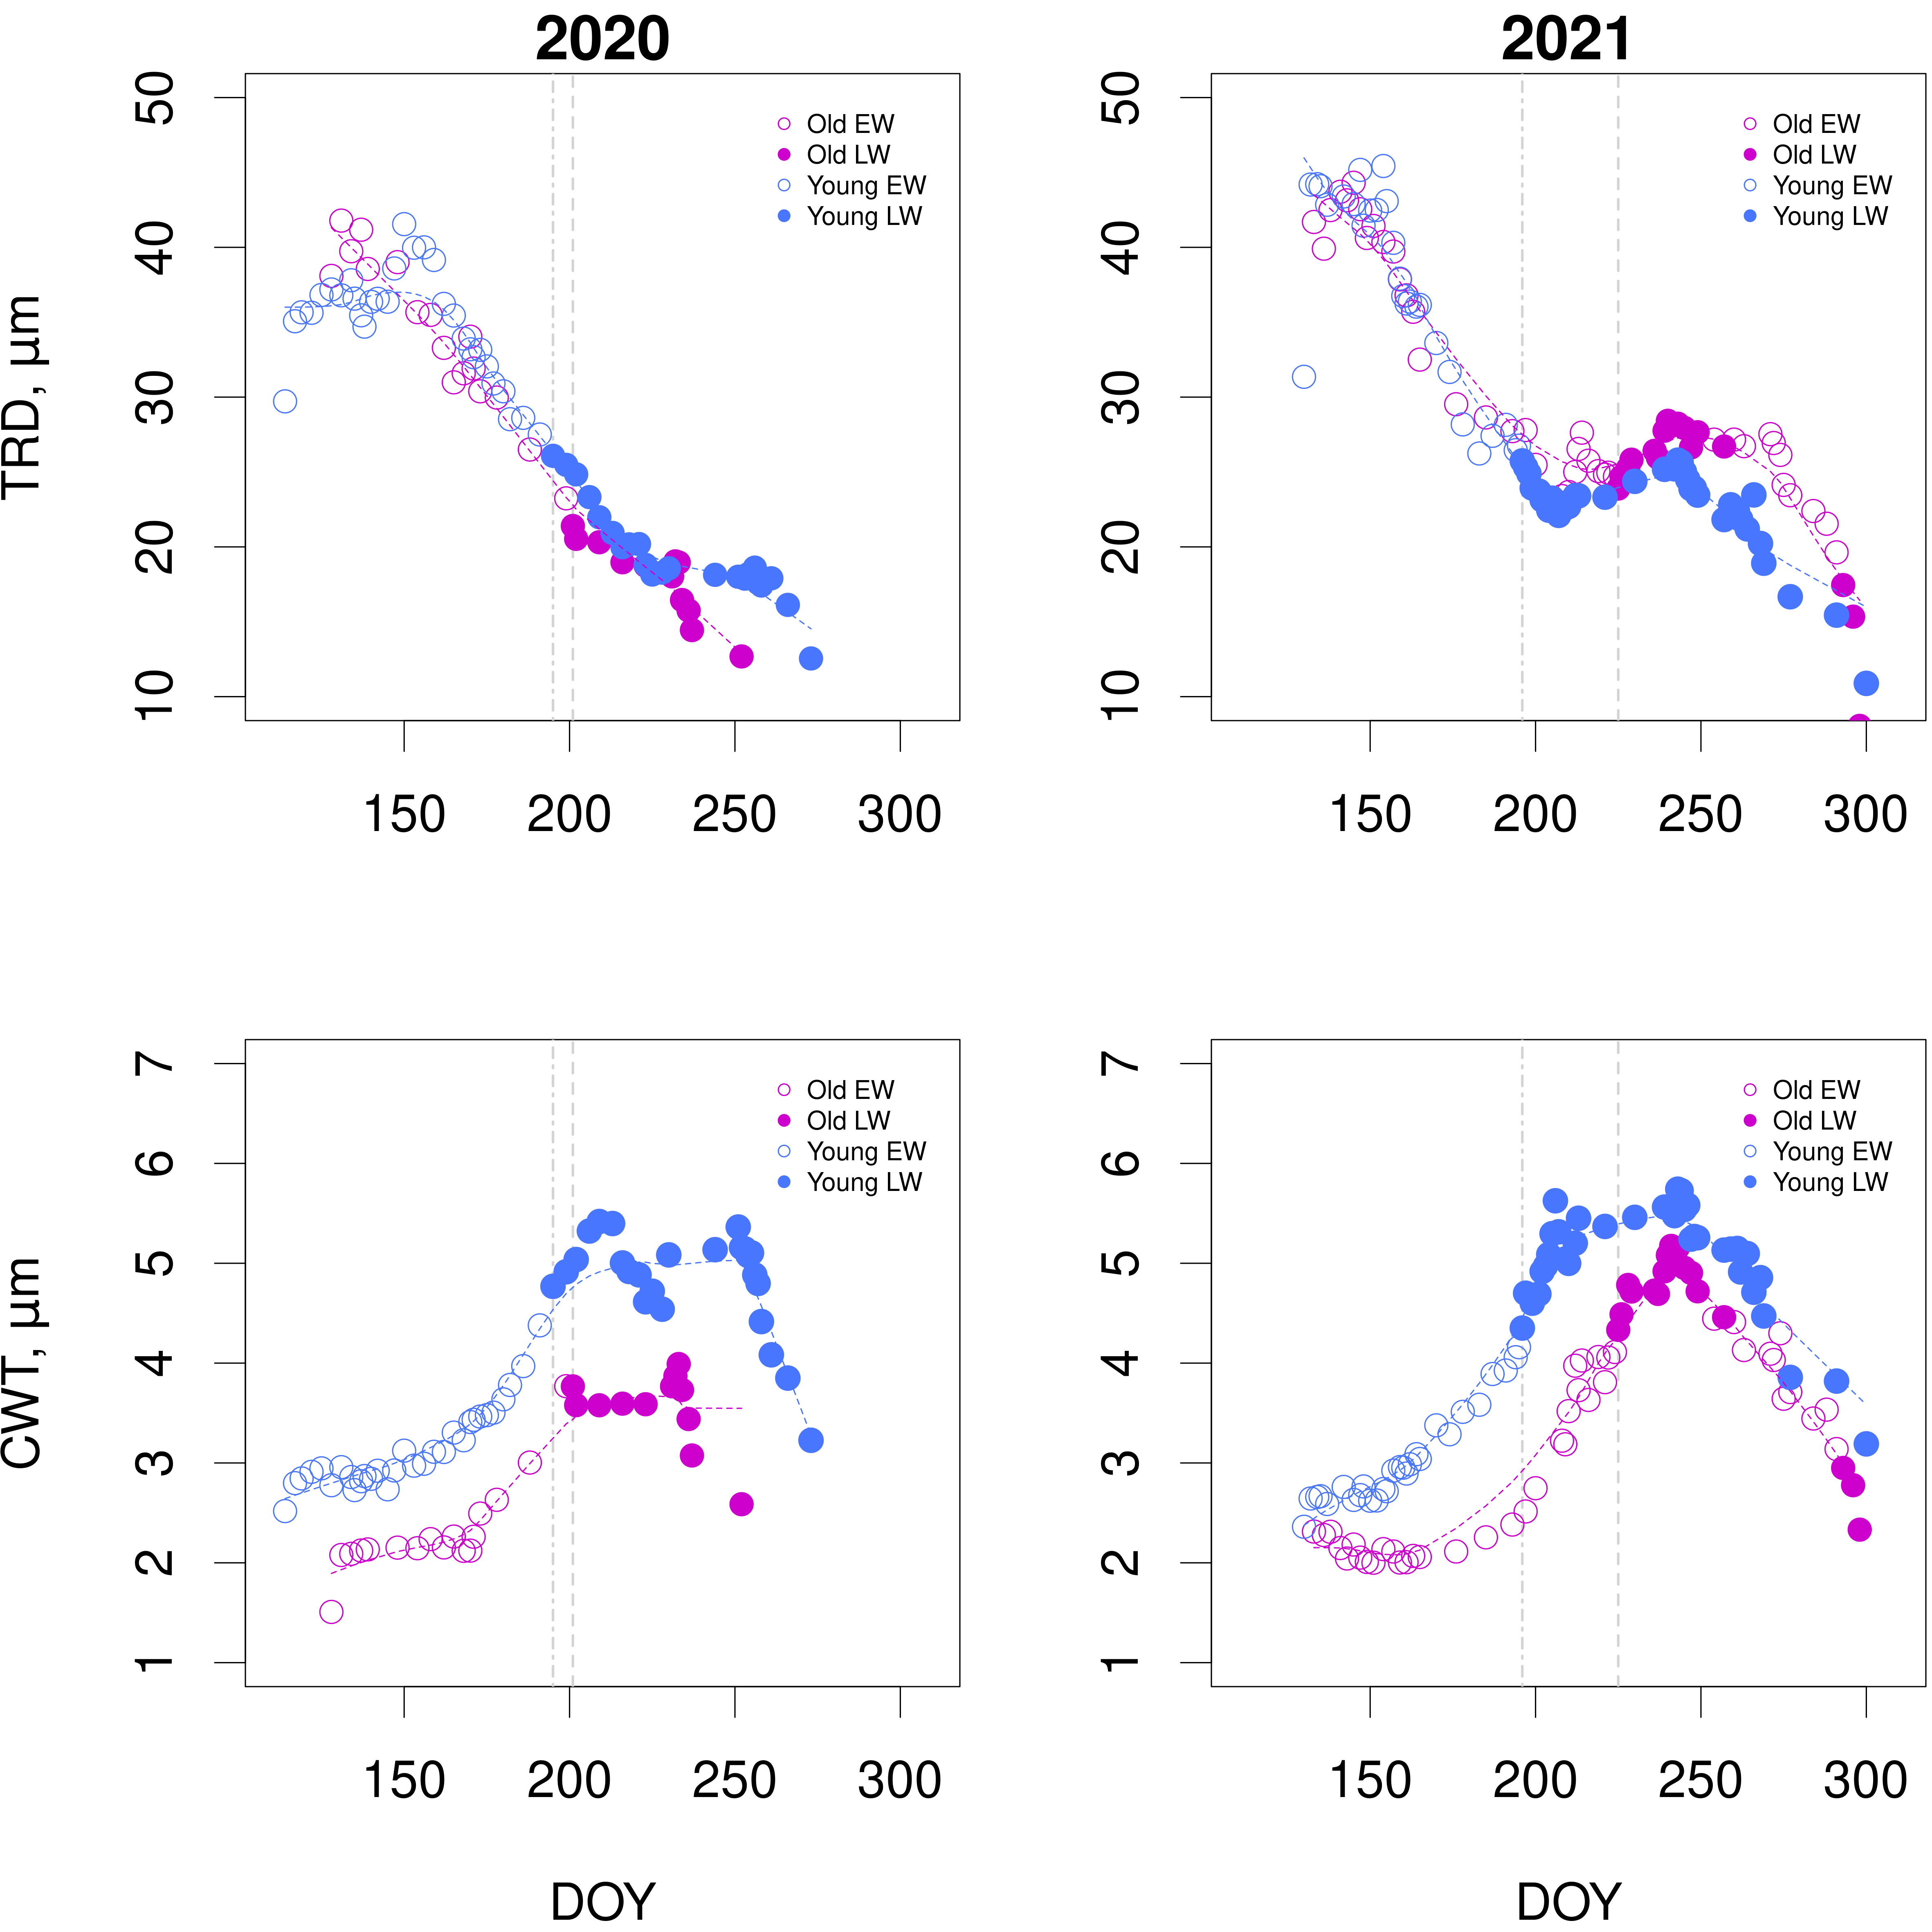
\includegraphics[width=1\textwidth]{pics/xmg}
                \caption{TRD -- tracheid radial diameter, CWT -- cell wall thickness, DOY -- day of the beginning of cell wall thichening (thus, TRD has already been formed}
            \end{figure}
    \end{block}

	\end{column}

\end{columns}

\begin{columns}[c]
    \begin{column}{.96\paperwidth}

    \begin{block}{What is next?}
        \raggedleft
        \begin{itemize}
            \item To study wood formation in the next years and more pine plots
            \item To study mg and dh on the upper limit of species distribution
        \end{itemize}
    \end{block}
\end{column}

\separatorcolumn

\end{columns}
\end{frame}

\end{document}
